\documentclass[letterpaper, 12pt]{report}
\usepackage[utf8]{inputenc}
\usepackage{amsmath,amssymb,amsthm}
\usepackage[spanish]{babel}
\usepackage{graphicx}
\usepackage{caption}
\usepackage{subcaption}
\usepackage{xcolor}
\usepackage{titlesec}
\usepackage{lmodern}
\usepackage{fancyhdr}
\usepackage{geometry}
\usepackage{algorithm}
\usepackage{algpseudocode}
\usepackage{multirow}
\usepackage{booktabs}
\usepackage{listings}
\usepackage{enumitem}

% Paradoja de pooling

\hyphenpenalty=10000 % Penaliza fuertemente la división de palabras
\exhyphenpenalty=10000 % Penaliza división después de guiones existentes
\tolerance=1 % Reduce la "urgencia" de dividir palabras
\emergencystretch=\maxdimen % Evita overfull boxes sin dividir palabras


\definecolor{codegreen}{rgb}{0,0.6,0}
\definecolor{codegray}{rgb}{0.5,0.5,0.5}
\definecolor{codepurple}{rgb}{0.58,0,0.82}


\setlength{\headheight}{24.01996pt}
\addtolength{\topmargin}{-12.01996pt}

% Definir colores personalizados
\definecolor{primary}{RGB}{25,55,95}
\definecolor{secondary}{RGB}{200,35,45}

% Configurar márgenes
\geometry{
    left=3cm,
    right=2.5cm,
    top=3cm,
    bottom=2.5cm
}

\newtheorem*{theorem*}{Teorema}

% Configurar estilo de títulos
\titleformat{\chapter}[display]
{\normalfont\Huge\bfseries\color{primary}}
{\chaptertitlename\ \thechapter}{20pt}{\Huge}

\titleformat{\section}
{\normalfont\Large\bfseries\color{primary}}
{\thesection}{1em}{}

% Configurar encabezado y pie de página
\pagestyle{fancy}
\fancyhf{}\hyphenpenalty=10000 % Penaliza fuertemente la división de palabras
\exhyphenpenalty=10000 % Penaliza división después de guiones existentes
\tolerance=1 % Reduce la "urgencia" de dividir palabras
\emergencystretch=\maxdimen % Evita overfull boxes sin dividir palabras
\fancyhead[L]{\small\textcolor{primary}{\nouppercase{\leftmark}}}
\fancyfoot[C]{\textcolor{primary}{\thepage}}
\renewcommand{\headrulewidth}{0.4pt}
\renewcommand{\headrule}{\hbox to\headwidth{\color{primary}\leaders\hrule height \headrulewidth\hfill}}

% Portada personalizada
\newcommand*{\customtitlepage}{
    \begin{titlepage}
        \begin{center}
            \vspace*{1cm}
            
            
            {\LARGE \textbf{UNIVERSIDAD DE LA HABANA}}\\
            \vspace{0.5cm}
            {\Large Facultad de Matem\'atica y Computaci\'on}\\
            

            
\includegraphics[scale=0.5]{images/logo.png}
            
            \vspace{1cm}
            
            
            \rule{\textwidth}{1.5pt}\\
            \vspace{0.5cm}
            {\LARGE \textcolor{primary}{\textbf{Primer Proyecto de Simulación}}}
            \vspace{0.5cm}
            \rule{\textwidth}{1.5pt}
            
            \vspace{2cm}
            
            {\Large \textbf{Servidores Especializados vs Servidores Generalistas}}\\
            \vspace{1cm}
            
            {\Large \textbf{Autor:} Lidier Robaina Caraballo \\
            \vspace{0.5cm}
            {\Large \textbf{Grupo:} C-411 }\\
            \vspace{1.5cm}
            
            {\Large 13 de abril de 2025
            }
            }
        \end{center}
    \end{titlepage}
}

\begin{document}

\customtitlepage

% Índice
\tableofcontents
\thispagestyle{empty}
\cleardoublepage

% Contenido principal
\setcounter{page}{1}

\chapter{Introducción}



En el ámbito de la gestión de servicios, la elección entre estrategias especializadas (recursos dedicados a tareas específicas) y generalistas (recursos multifuncionales) constituye un dilema recurrente. La eficiencia del proceso y la experiencia del usuario están directamente vinculadas a cómo se estructuran los recursos disponibles \cite{pinker2000} . Este proyecto aborda dicho desafío mediante la simulación basada en eventos discretos, una técnica que permite modelar sistemas dinámicos con precisión bajo condiciones controladas y replicables. \\



El estudio compara dos modelos de colas contrastantes:

\begin{enumerate}
    \item[\textbf{a)}] Escenario especializado   \begin{itemize}[noitemsep]
        \item Servidores dedicados a un único tipo de tarea.
        \item \textit{Configuración de colas}: Múltiples colas dedicadas (una por tipo de demanda).
        \item \textit{Riesgo clave}: Costos asociados a desequilibrio de ocupación entre colas.
    \end{itemize}
    
    \item[\textbf{b)}] Escenario generalista
    \begin{itemize}[noitemsep]
        \item Servidores flexibles que atienden múltiples demandas.
        \item \textit{Configuración de colas}: Cola única atendida por todos los servidores.
        \item \textit{Riesgo clave}: Incremento del tiempo de atención por cambios de contexto.
    \end{itemize}
\end{enumerate}


Aunque el análisis se desarrolla en un caso simplificado de una sucursal bancaria (procesos de retiros y depósitos), los hallazgos buscan extrapolarse a sistemas complejos como cadenas logísticas, centros de atención al cliente o redes hospitalarias.

\section{Objetivos y metas}
El objetivo principal es evaluar comparativamente el desempeño de ambas estrategias, con tres metas específicas:

\begin{itemize}
    \item[1.] Cuantificar la eficiencia global mediante métricas fundamentales.  
    \item[2.] Evaluar \textit{trade-off}  entre eficiencia y resiliencia.
    \item[3.] Generar recomendaciones basadas en evidencia para optimizar sistemas de servicios.
\end{itemize}


\section{Sistema específico a simular}

El texto del problema fue extraído de \cite{sabater2015} \footnote{Problema Gasto de recursos por desequilibrio6.5: Sucursal Bancaria.}.

\begin{quote}
    Una pequeña sucursal de un banco tiene dos empleados, uno para los pagos y otro para los cobros. Los clientes llegan a 
cada caja siguiendo una distribución de Poisson con una media de 20/hora (el total de llegada al banco es de 40/hora). 
El tiempo de servicio de cada empleado es una negativa exponencial de media 2 minutos. El encargado de la sección está 
pensando hacer un cambio en que los dos operarios puedan hacer tanto pagos como cobros para evitar situaciones en que 
una cola está llena y la otra parada. Sin embargo, se estima que cuando los empleados se encarguen de las dos cosas 
el tiempo de servicio aumentará a una media de 2,4 minutos. Compara el sistema que se emplea ahora con el propuesto, 
calculando el total de gente en el banco, el tiempo medio que pasaría un cliente en el banco hasta que es atendido, 
la probabilidad de que un cliente espere más de cinco minutos y el tiempo medio que están parados los empleados. 
\end{quote}

Se tienen las siguientes variables de interés:
\begin{itemize}
    \item \textbf{L:} Media del total de clientes en el sistema en cada instante (congestión del sistema)
    \item \(\mathbf{W_q}\)\textbf{:} Media del tiempo durante el que un cliente permanece en la cola (tiempo de espera)
    \item \(\mathbf{P ( W_q > t_{max})}\)\textbf{:} Probabilidad de que el tiempo de espera de un cliente sea superior a un tiempo determinado (retrasos críticos)
    \item \(\mathbf{P_{idle}}\)\textbf{:} Porcentaje del tiempo durante el cual los servidores no tienen clientes (capacidad ociosa)  
\end{itemize}


\section{Variables que describen el problema}

\begin{itemize}
    \item \(\mathbf{\lambda_1}\)\textbf{:} tasa media de llegadas por hora de clientes para pagos (distribución de Poisson con parámetro $\lambda_1$)
    \item \(\mathbf{\lambda_2}\)\textbf{:} tasa  media de llegadas por hora de clientes para cobros (distribución de Poisson con parámetro $\lambda_2$)    
    \item \(\mathbf{t_1}\)\textbf{:} media del tiempo (minutos) de atención en el servidor 1 (distribución exponencial con frecuencia $\mu_1 = \frac{60}{t_1}$ clientes atentidos por hora)
    \item \(\mathbf{t_2}\)\textbf{:} media del tiempo (minutos) de atención en el servidor 2 (distribución exponencial con frecuencia $\mu_2 = \frac{60}{t_2}$ clientes atendidos por hora)
    \item \(\mathbf{t_{max}}\)\textbf{:} tiempo (minutos) de espera crítico 
\end{itemize}

En caso de escenario especializado, el servidor 1 atiende los pagos y el servidor 2 los cobros. En caso de escenario generalista, $t_1 = t_2$.



\chapter{Implementación}

\section{Detalles de implementación}


\begin{itemize}
    \item[\textbf{1.}] \textbf{Gestión de Eventos:}
    Se emplea una cola de prioridad (módulo \texttt{heapq}) para manejar la lista cronológica de eventos. Cada evento contiene:
    \begin{itemize}
        \item Marca temporal de ejecución
        \item Tipo (llegada o salida)
        \item Metadatos específicos (índice de servidor/cola)
    \end{itemize}
    
    \item[\textbf{2.}] \textbf{Estructuras de Datos:}
    \begin{itemize}
        \item \textbf{Colas de espera}: Arreglos separados para cada servicio en modo especializado vs cola única compartida en modo generalista
        \item \textbf{Estado de servidores}: Arreglo booleano que indica disponibilidad
        \item \textbf{Contadores de clientes}: Registro separado por colas (especializado) o contador único (generalista)
    \end{itemize}
    
    \item[\textbf{3.}] \textbf{Mecánica de Simulación:}
    \begin{itemize}
        \item \textbf{Llegadas}: Generadas mediante proceso Poisson usando \texttt{random.expovariate()}
        \item \textbf{Tiempos de servicio}: Modelados con distribución exponencial negativa
        \item \textbf{Asignación de servidores}: Política FIFO con prioridad a servidores disponibles
    \end{itemize}
    
    \item[\textbf{4.}] \textbf{Recolección de Métricas:}
    \begin{itemize}
        \item \textit{Área acumulativa} para cálculos promediados en el tiempo
        \item Lista de tiempos de espera individuales
        \item Registro de ocupación de servidores
        \item Cálculo final mediante integración temporal (método de área bajo la curva)
    \end{itemize}
\end{itemize}

\section{Pasos de la simulación}


El flujo de ejecución sigue esta secuencia lógica:

\begin{enumerate}[leftmargin=1.5cm]
    \item \textbf{Inicialización:}
    \begin{itemize}
        \item Crear estructura de colas según estrategia
        \item Programar primeros eventos de llegada usando tasas $\lambda_1$ y $\lambda_2$
        \item Inicializar contadores y registros estadísticos
    \end{itemize}
    
    \item \textbf{Bucle Principal de Eventos:}
    \begin{lstlisting}[language=Python]
    while time < sim_time:
        event = heappop(events)
        actualizar_estadisticas()
        procesar_evento(event)
    \end{lstlisting}
    
    \item \textbf{Procesamiento de Llegadas:}
    \begin{itemize}
        \item Insertar cliente en la cola correspondiente
        \item Si hay servidor disponible:
        \begin{itemize}
            \item Iniciar servicio inmediato
            \item Registrar tiempo de espera cero
            \item Programar evento de salida
        \end{itemize}
        \item Generar próxima llegada según distribución Poisson
    \end{itemize}
    
    \item \textbf{Manejo de Salidas:}
    \begin{itemize}
        \item Liberar servidor
        \item Si existen clientes en cola:
        \begin{itemize}
            \item Extraer siguiente cliente
            \item Calcular tiempo de espera (current\_time - arrival\_time)
            \item Programar nuevo evento de salida
        \end{itemize}
    \end{itemize}
    
    \item \textbf{Actualización Estadística:}
    \begin{itemize}
        \item Calcular tiempo transcurrido desde último evento
        \item Acumular:
        \begin{itemize}
            \item Clientes-tiempo en sistema
            \item Tiempo ocupado de servidores
        \end{itemize}
        \item Mantener precisión temporal mediante integración continua
    \end{itemize}
    

\end{enumerate}

\chapter{Resultados y experimentos}

\section{Variables de interés}

Se ejecutaron 1000 simulaciones independientes para cada configuración del sistema. Para cada métrica, se comparan las distribuciones resultantes de ambas estrategias mediante el histograma normalizado y la distribución normal correspondiente a la media y desviación estándar de los datos.

\subsection{Análisis exploratorio}

\begin{figure}[H]
    \centering
    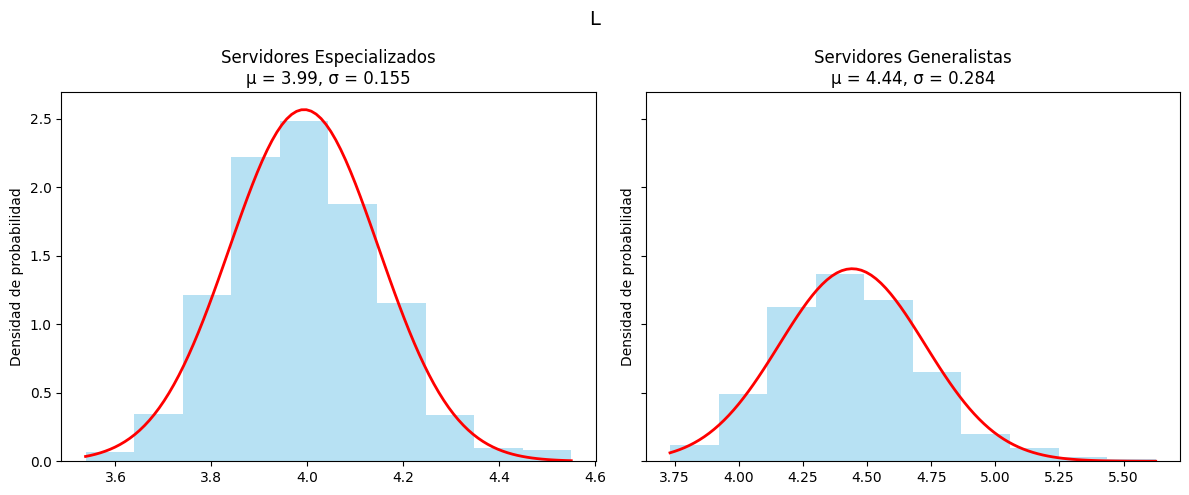
\includegraphics[width=0.95\textwidth]{images/L.png}
    \caption{Histograma de la media de clientes en el sistema ($L$)}
    \label{fig:clientes}
\end{figure}


\begin{figure}[H]
    \centering
    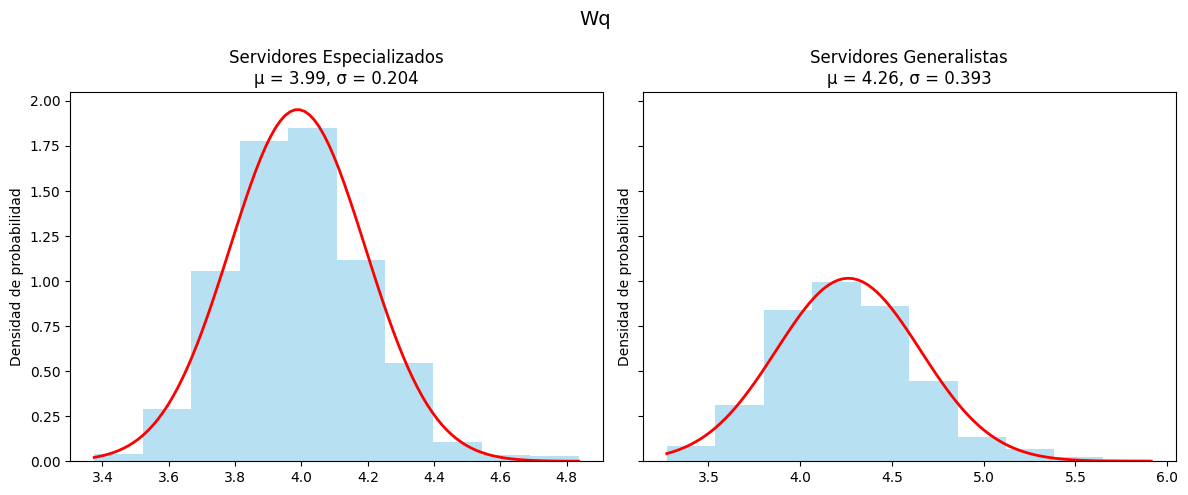
\includegraphics[width=0.95\textwidth]{images/Wq.png}
    \caption{Histograma del tiempo (min) medio de espera ($W_q$)}
    \label{fig:espera}
\end{figure}

\vspace{2cm}

\begin{figure}[H]
    \centering
    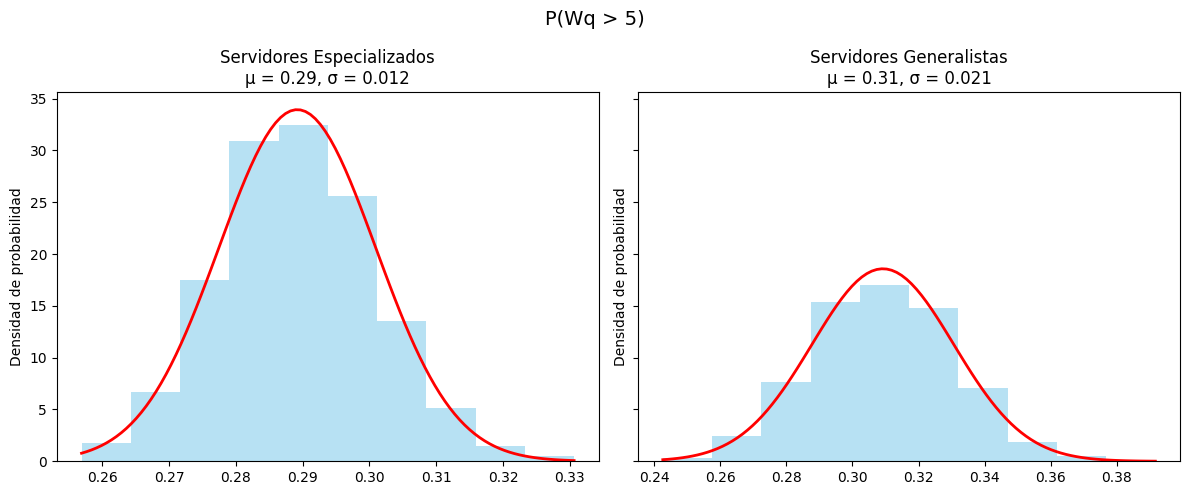
\includegraphics[width=0.95\textwidth]{images/PWqovertk.png}
    \caption{Histograma de la probabilidad de superar el umbral de 5 minutos de espera}
    \label{fig:probabilidad}
\end{figure}


\begin{figure}[H]
    \centering
    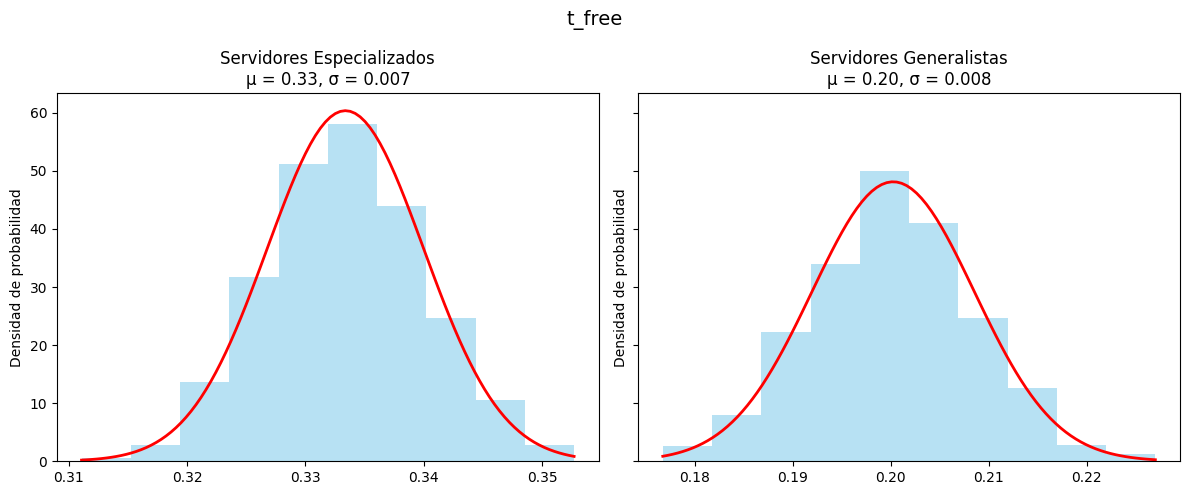
\includegraphics[width=0.95\textwidth]{images/tfree.png}
    \caption{Histograma de la tasa de tiempo inactivo de los servidores}
    \label{fig:inactividad}
\end{figure}

\subsection{Interpretación de los resultados}

\begin{itemize}
    \item Al seguir una estrategia generalista, aunque se distribuye la carga entre dos servidores, el tiempo de servicio por cliente aumenta debido
    a la reducci\'on de la especialización. Por tango, aumenta la congestión del sistema y el tiempo de espera de los usuario.
    \item La probabilidad de retrasos críticos no difiere significativamente, debido a que la distribución exponencial mitiga los efectos de las diferencias en las probabilidades de cola larga.
    \item En el sistema especializado, los servidores no pueden redistribuir la carga. Si una cola está vacía, su servidor permanece inactivo aunque haya demanda en la otra cola, por tanto tiene un peor uso de recursos.
\end{itemize}

\subsection{Hipótesis extraídas}

\subsubsection{Hipótesis 1: Mayor congestión de clientes en sistema generalista}
\begin{itemize}
    \item \textbf{Hipótesis nula:} $H_0: \mu_{\text{propuesto}} \leq \mu_{\text{actual}}$ 
    \item \textbf{Hipótesis alternativa:} $H_1: \mu_{\text{propuesto}} > \mu_{\text{actual}}$ 
\end{itemize}

\subsubsection{Hipótesis 2: Mayor tiempo de espera en sistema generalista}
\begin{itemize}
    \item \textbf{Hipótesis nula:} $H_0: W_{\text{propuesto}} \leq W_{\text{actual}}$ 
    \item \textbf{Hipótesis alternativa:} $H_1: W_{\text{propuesto}} > W_{\text{actual}}$ 
\end{itemize}

\subsubsection{Hipótesis 3: Similar probabilidad de retrasos críticos}
\begin{itemize}
    \item \textbf{Hipótesis nula:} $H_0: p_{\text{actual}} = p_{\text{propuesto}}$ 
    \item \textbf{Hipótesis alternativa:} $H_1: p_{\text{actual}} \neq p_{\text{propuesto}}$ 
\end{itemize}


\subsubsection{Hipótesis 4: Mayor inactividad en sistema especializado}
\begin{itemize}
    \item \textbf{Hipótesis nula:} $H_0: I_{\text{actual}} \leq I_{\text{propuesto}}$ 
    \item \textbf{Hipótesis alternativa:} $H_1: I_{\text{actual}} > I_{\text{propuesto}}$ 
\end{itemize}

\subsection{Pruebas de Hipótesis}

Se realiz\'o un test t-student para cada hipótesis, en todos los casos se 
obtuvieron p-values muy cercanos a 0, así que en todos los casos
se rechaza la hipótesis nula. Se puede asegurar que hay diferencias significativas
en la media de cada variable para las dos estrategias.

\chapter{Modelo matemático}


\section{Descripción del modelo}

La teoría de colas analiza sistemas de espera mediante procesos estocásticos. En sistemas markovianos $M/M/c$, se asumen procesos Poisson de llegada con tasa $\lambda$ y servicio con tasa $\mu$, lo que permite modelar el sistema de nuestro problema como una cadena de Markov en tiempo continuo. \\

Definimos:
\begin{itemize}
\item $c:$ Número de servidores en paralelo
    \item $\rho = \frac{\lambda}{c\mu} :$ Factor de utilización de cada servidor
    \item $r = \frac{\lambda}{\mu} :$ Número promedio de clientes que atienden en conjunto los servidores cada instante
    \item $L$: Número promedio de clientes en el sistema
    \item $L_q$: Longitud promedio de la cola
    \item $W$: Tiempo promedio en el sistema
    \item $W_q$: Tiempo promedio en cola
    \item $P_0$: Probabilidad de sistema vacío
    \item $P_{idle}$: Probabilidad de que un servidor no tenga clientes (capacidad ociosa)
    
\end{itemize}
    
Estas métricas clave se obtienen resolviendo ecuaciones de balance y aplicando la \textbf{Ley de Little}: $L=\lambda W$. En esta sección, las f\'ormulas que no est\'an explícitamente justificadas fueron obtenidas de \cite{sabater2015}.  
    


\subsection{Sistema Especializado}

Para cada servidor simple independiente ($\lambda=20$, $\mu=30$), aplicamos el modelo $M/M/1$.


\begin{itemize}
    \item Clientes en sistema  
    \begin{flalign*}
\rho &= \frac{\lambda}{\mu} = \frac{2}{3} & \\
L &= \frac{\rho}{1 - \rho} = 2 \text{\ por servidor} \Rightarrow \text{4 en total} &
\end{flalign*}

 
    \item Tiempo de espera    
 \begin{flalign*}
W_q &= \frac{\rho}{\mu - \lambda} = \frac{2}{30} \text{\ horas} = 4 \text{\ minutos} &
\end{flalign*}

\item Probabilidad de retraso cr\'itico

En \cite{book} se demuestra que el tiempo de espera en cola de un sistema $M/M/c$ se comporta seg\'un la siguiente distribuci\'on exponencial modificada:
 \begin{flalign*}
P(W_q \leq t) &= 1 - P_w \ e^{-(c\mu - \lambda)t} &
\end{flalign*}
donde $P_w$ es la probabilidad de que el sistema est\'e lleno y el cliente tenga que esperar al llegar. En este caso $P_w = \rho$, por tanto:
\begin{flalign*}
P(W_q > t) &= 1 - P(W_q \leq t) = \rho e^{-(\mu - \lambda)t} & \\ 
P(W_q > 5) &= P(W_q > \frac{1}{12} \ \text{horas}) = \frac{2}{3} e^{-10\frac{1}{12}} \approx 0.2897    &
\end{flalign*}

\item Capacidad ociosa
 \begin{flalign*}
P_{idle} &= 1 - \rho = \frac{1}{3} &
\end{flalign*}

\end{itemize}



\subsection{Sistema Generalista}


Para el sistema conjunto de los dos servidores en paralelo ($\lambda=40$, $\mu=25$, $c=2$), aplicamos el modelo $M/M/2$.


\begin{itemize}
    \item Clientes en sistema  
    \begin{flalign*}
\rho &= \frac{\lambda}{c\mu} = \frac{4}{5} & \\
r &= \frac{\lambda}{\mu} = \frac{8}{5} & \\
P_0 &= \left[\sum_{n=0}^{c-1}\frac{r^n}{n!} + \frac{r^c}{c!(1-\rho)}\right]^{-1} = \left[1 + r + \frac{r^4}{0.4} \right]^{-1} = \frac{1}{9} &  \\
L_q &= \frac{r^c\rho}{c!(1-\rho)^2}P_0 = \frac{2.56 \cdot 0.8}{2 \cdot 0.04 \cdot 9} = 2.8444 \ \ \Rightarrow \ \  L = L_q + r = 4,4444 & 
\end{flalign*}

 
    \item Tiempo de espera  \\
      
    Aplicando Ley de Little:
      \begin{flalign*}
W_q &= \frac{L_q}{\lambda} = 0.07111 \text{\ horas} \approx 4,2667 \text{\ minutos}  &
\end{flalign*}

\item Probabilidad de retraso cr\'itico

En este caso, $P_w = \frac{r^cP_0}{c!(1-\rho)}$, luego:
\begin{flalign*}
P(W_q > t)  &= 1 - P(W_q \leq t) = \frac{r^cP_0}{c!(1-\rho)}e^{-(c\mu - \lambda)t} & \\
P(W_q > 5) &= P(W_q > \frac{1}{12} \ \text{horas}) = \frac{2.56 \cdot \frac{1}{9}}{2 \cdot 0.2} e^{-10\frac{1}{12}} \approx 0.3090  &
\end{flalign*}

\item Capacidad ociosa
 \begin{flalign*}
P_{idle} &= 1 - \rho = \frac{1}{5} &
\end{flalign*}

\end{itemize}





\section{Supuestos y restricciones}
\begin{itemize}

    \item    \textbf{Proceso de nacimiento-muerte:} Las transiciones entre estados siguen una cadena de Markov con tasas $\lambda$ (nacimientos) y $\mu$ (muertes). Los servidores se comportan de forma id\'entica.

   \item  \textbf{Equilibrio estable:} $\rho<1$ garantiza estado estacionario ($\rho=0.6667$ y $\rho=0.8$ cumplen esto).     
    

    \item \textbf{Política FIFO:} Clientes son atendidos en orden de llegada
    

    \item \textbf{Independencia:} Llegadas y servicios son procesos independientes
   \item \textbf{Memoria exponencial:} Los tiempos entre llegadas y servicios carecen de memoria, justificando el uso de distribuciones exponenciales.   
   
    \item \textbf{Espacio infinito:} Capacidad ilimitada en las colas
    \item \textbf{Homogeneidad:} Tasas constantes en el tiempo
    
    
\end{itemize}



\newpage


\section{Comparación de resultados}
\begin{table}[h]
\centering
\caption{Resultados Teóricos vs. Experimentales}
\begin{tabular}{cccccc}
\toprule
\textbf{Métrica} & \multicolumn{2}{c}{\textbf{Especializado}} & \multicolumn{2}{c}{\textbf{Generalista}} \\
 & Teórico & Experimental & Teórico & Experimental \\
\midrule
Clientes en el sistema & 4 & 3.99 & 4.4444 & 4.44 \\
Tiempo en cola (min) & 4 & 3.99 & 4.2667 & 4.26 \\
Prob. de retraso crítico & 0.2897 & 0.29 & 0.3090 & 0.31 \\
Tiempo inactivo (\%) & 33 & 33 & 20 & 20 \\
\bottomrule
\end{tabular}
\end{table}

La concordancia de resultados (error $< 1 \%$) confirma los supuestos markovianos y la aplicabilidad del modelo. Se observa que ambos enfoques proveen una base s\'olida para la toma de decisiones operarivas.

\chapter{Conclusiones}



\begin{itemize}
\item[1.] \textbf{Eficiencia cuantificada:}

\begin{itemize}
\item El sistema especializado presenta mejor desempeño operativo inmediato  gracias a su menor factor de utilización, pero con mayor capacidad ociosa.
\item El sistema generalista logra mayor eficiencia agregada al compartir recursos, pero con penalización en la congesti\'on y los tiempos de espera.
\end{itemize}



\item[2.] \textbf{Trade-off entre eficiencia y resiliencia:} 

\begin{itemize}
 \item   El sistema especializado prioriza la rapidez en atención individual, pero su alta tasa de inactividad lo hace vulnerable a fluctuaciones en la demanda. 

\item   El sistema generalista, aunque presenta tiempos de espera mayores, garantiza mayor resiliencia al distribuir la carga entre servidores, reduciendo drásticamente la probabilidad de colapsos. 
\end{itemize}



\item[3.] \textbf{Recomendaciones estratégicas:}
La elección óptima depende del contexto operativo:
\begin{itemize}

    
    \item \textbf{Especializado} recomendable cuando:

    Los servicios tienen alta priorización de tiempos de respuesta (ej.: atención médica urgente).

    La congesti\'on tiene consecuencias operativas severas. 
    
\item \textbf{Generalista} preferible cuando:

   Los sistemas tienen demanda variable o alta incertidumbre.
   
    Los costes de capacidad ociosa superan los de congestión marginal.    
    
    \item \textbf{Solución híbrida} propuesta: Mantener especialización base + servidores generalistas flotantes para absorber picos de demanda.
    \end{itemize}
    \end{itemize}



Este análisis demuestra que no existe una solución universal óptima, sino configuraciones adaptativas donde la arquitectura de colas debe alinearse con los parámetros críticos del negocio y el perfil de riesgo organizacional.

\begin{thebibliography}{9}

    \bibitem{pinker2000} Pinker, E. J., \& Shumsky, R. A. (2000). The efficiency-quality trade-off of cross-trained workers. Manufacturing \& Service Operations Management, 2(1), 32-48.

    \bibitem{sabater2015} Sabater, J. P., \& ROGLE, G. (2015). Aplicando Teoría de Colas en dirección de operaciones.
    
   \bibitem{book} Gross, D., Shortle, J. F., Thompson, J. M., \& Harris, C. M. (2011). Fundamentals of queueing theory (Vol. 627). John wiley \& sons.

%    
%    \bibitem{hu2022} Hu, J., Andradóttir, S., \& Ayhan, H. (2022). Server coordination in queueing systems: When and how?. Probability in the Engineering and Informational Sciences, 36(3), 868-922.
 
\end{thebibliography}




\end{document}
